% 1977 年四川卷第六题(1)：(x+2)(y-1)=0 的图象——直线 x=-2 与 y=1（按源卷第 5 页图一布局）
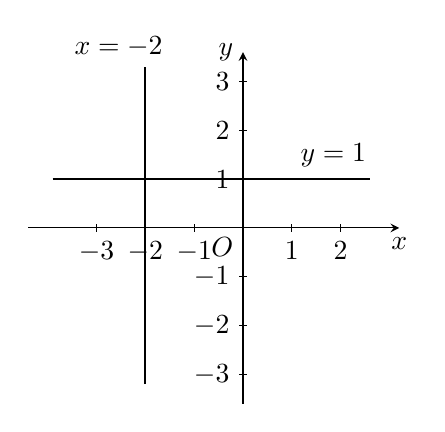
\begin{tikzpicture}[scale=0.62,>=stealth]
  \draw[->] (-4.4,0)--(3.2,0) node[below] {$x$};
  \draw[->] (0,-3.6)--(0,3.6) node[left] {$y$};
  \node[below left] at (0,0) {$O$};
  \foreach \x in {-3,-2,-1,1,2}{
    \draw[thin] (\x,0.08)--(\x,-0.08) node[below] {$\x$};
  }
  \foreach \y in {-3,-2,-1,1,2,3}{
    \draw[thin] (0.08,\y)--(-0.08,\y) node[left] {$\y$};
  }
  \draw[thick] (-2,-3.2)--(-2,3.3);
  \draw[thick] (-3.9,1)--(2.6,1);
  \node[above] at (-2.55,3.30) {$x=-2$};
  \node[above] at (1.85,1.04) {$y=1$};
\end{tikzpicture}
